\documentclass{article} 
\usepackage{amsmath} 
\usepackage{graphicx} 
\usepackage[top=1in, bottom=1in, left=.65in, right=.65in]{geometry} 
\usepackage{fancyhdr} 
\usepackage{multicol}
\usepackage{capt-of}
\usepackage[font=footnotesize,labelfont=bf]{caption}
\usepackage{siunitx}
\usepackage{tabularx}

%standard 2 column lab report template.

%scale = .22 for in/out plots
%scale = .4 for reg plots

%%%define figure environment, headers. remove section numbering.
\newenvironment{2colfig}{
  \par\medskip\noindent\minipage{\linewidth}
} {
  \endminipage\par\medskip
}

\newcommand{\labhead}[1]{
  \vspace{1em}
  {\bf #1}$_{\,}$
  \hline
  \vspace{1em}
}

\makeatletter
\newlength \figwidth
\if@twocolumn
  \setlength \figwidth {0.9\columnwidth}
\else
  \setlength \figwidth {0.5\textwidth}
\fi
\makeatother%

\setcounter{secnumdepth}{0}

\begin{document}
\lhead{PH 412 - Lab 8 rough.}
\chead{Rene Zeto} 
\rhead{\thepage} 
\pagestyle{fancy} 
\fancyfoot[c]{} 
\setlength{\parindent}{0pt}

\begin{multicols*}{2}
\labhead{7.1 Simple Comparator.}  
{\bf a.} We built the circuit using $V_b = +V_{cc} = \SI{8}{\volt}$. $R_1 = \SI{100}{\kilo\ohm}$. $R_2 = \SI{44.2}{\kilo\ohm}$ potentiometer.
\newline

\begin{2colfig}
  \center
  {\bf Comparator circuit.} \newline
  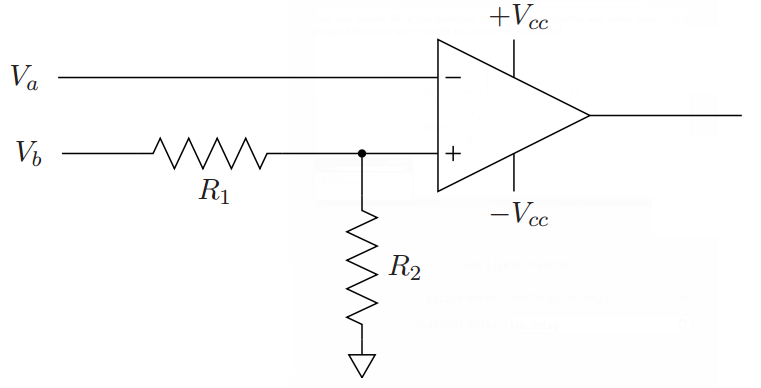
\includegraphics[scale=.4]{circuit1}
  \captionof{figure}{a simple figure. source: lab manual}\label{fig:circ1}
\end{2colfig}

{\bf b.} We applied a $V_a = \SI{10}{\volt}$ (peak to peak). $V_b = V_{cc}$ still. Scope traces below.

\begin{2colfig}
  \center
  {\bf Input and output signals.} \newline
  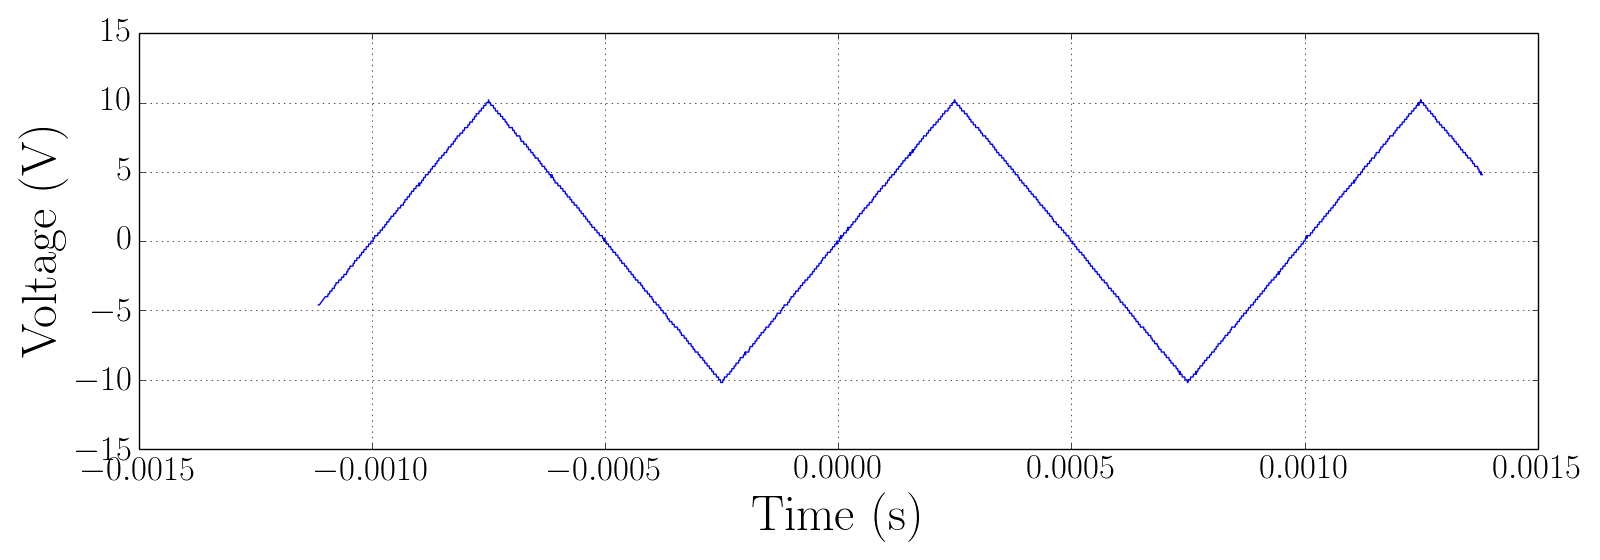
\includegraphics[scale=.22]{day1_lab8/ALL0000/F0000CH1}
  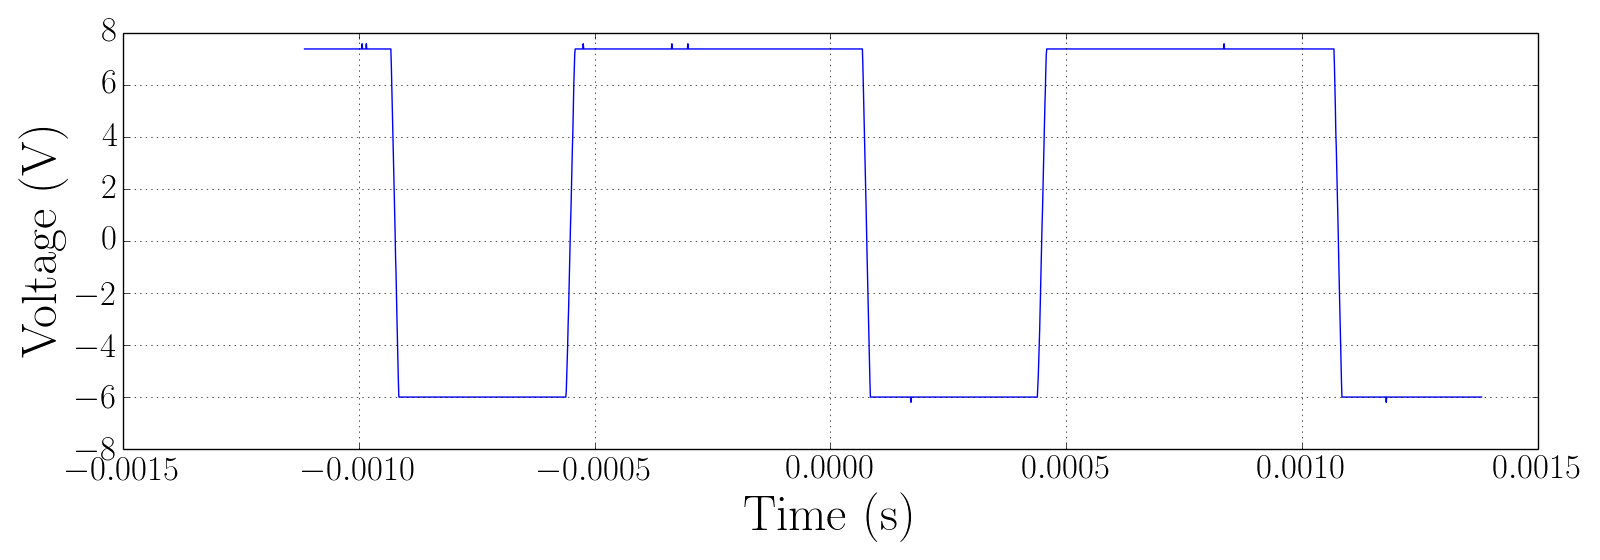
\includegraphics[scale=.22]{day1_lab8/ALL0000/F0000CH2}
  \captionof{figure}{a simple figure.}\label{fig:plot1}
\end{2colfig}

{\bf c.} We applied the same $v_a$ signal as in part b, but this time, we modulated it with \SI{50}{\kilo\hertz}, at
10\% depth. $V_b = V_{cc}$.

\begin{2colfig}
  \center
  {\bf Input and output signals.} \newline
  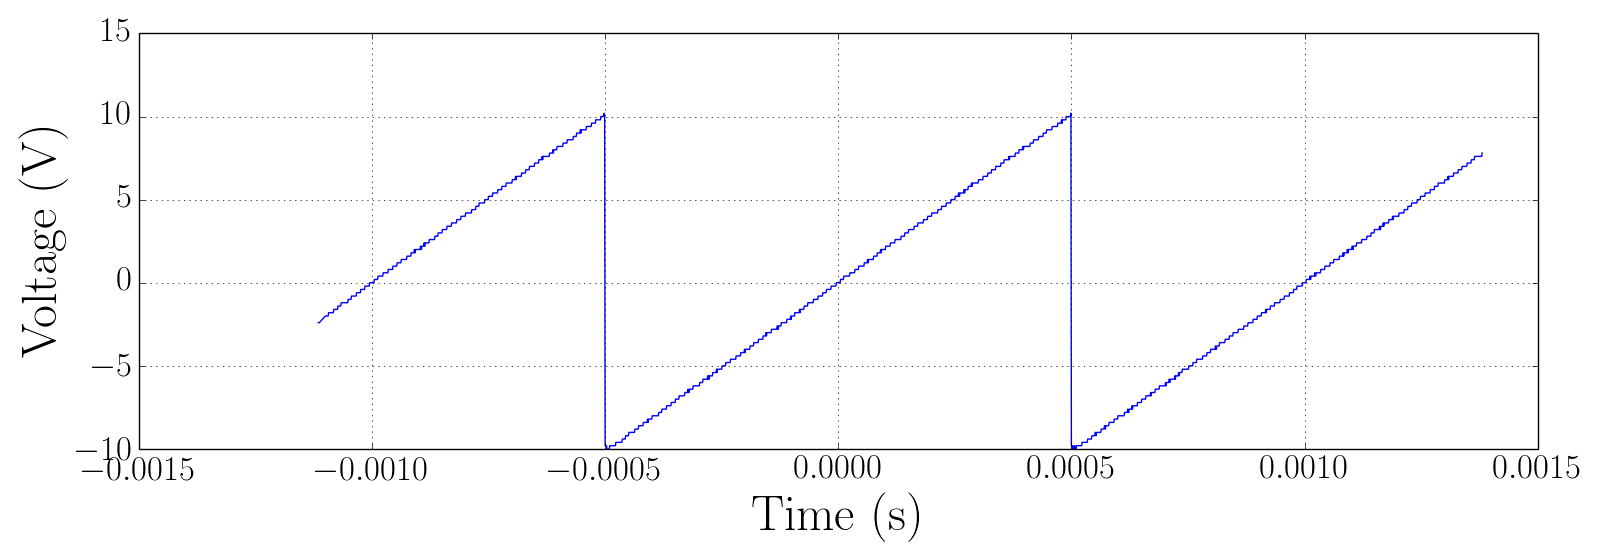
\includegraphics[scale=.22]{day1_lab8/ALL0001/F0001CH1}
  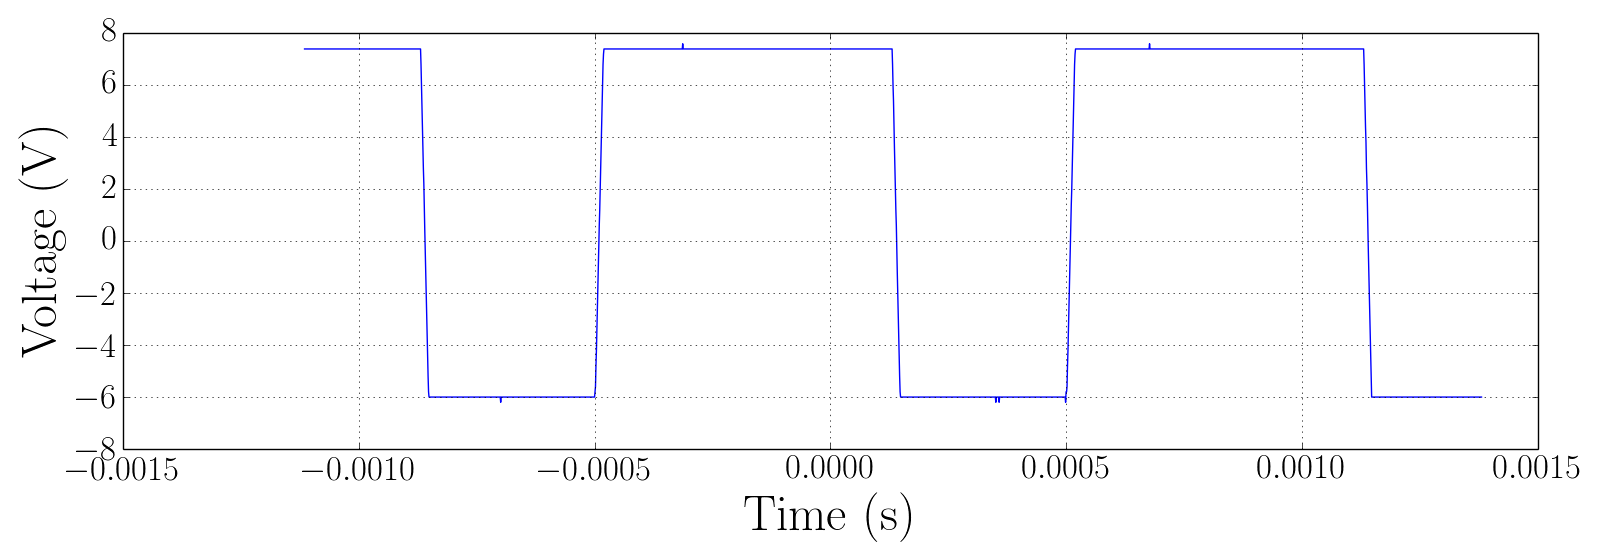
\includegraphics[scale=.22]{day1_lab8/ALL0001/F0001CH2}
  \captionof{figure}{a simple figure.}\label{fig:plot2}
\end{2colfig}

We then did it again, with \SI{10}{\kilo\hertz} modulation. 
\begin{2colfig}
  \center
  {\bf Input and output signals.} \newline
  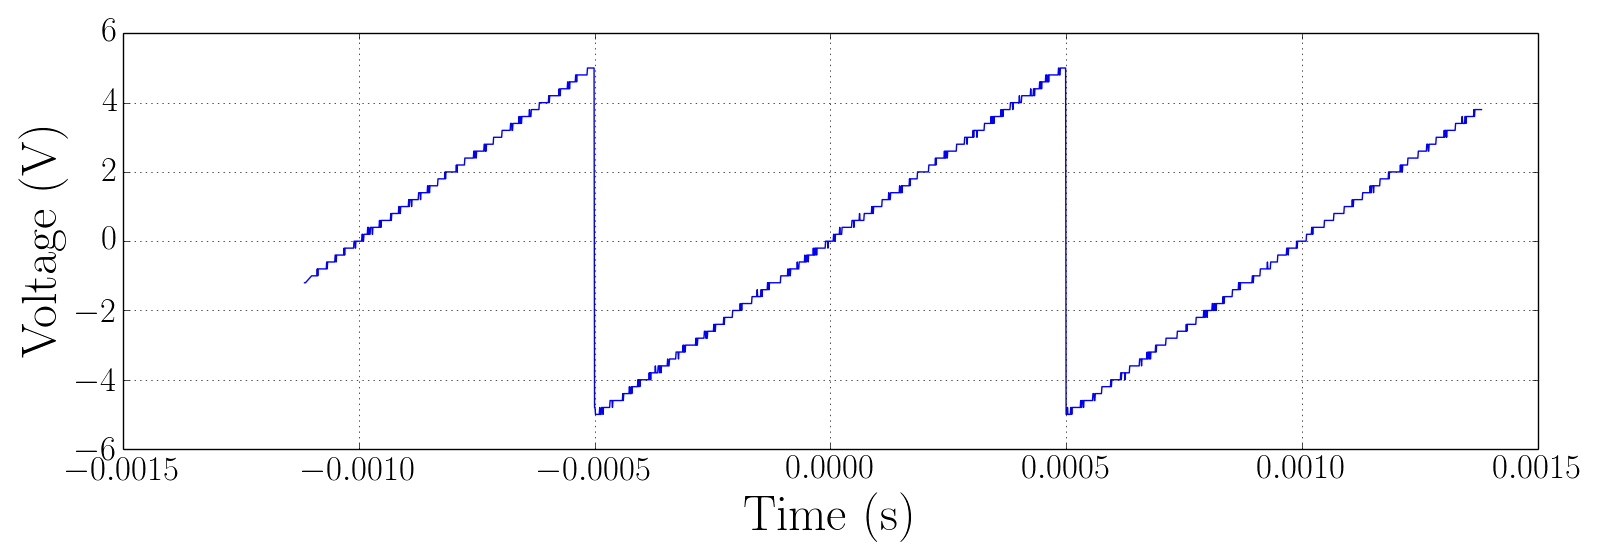
\includegraphics[scale=.22]{day1_lab8/ALL0002/F0002CH1}
  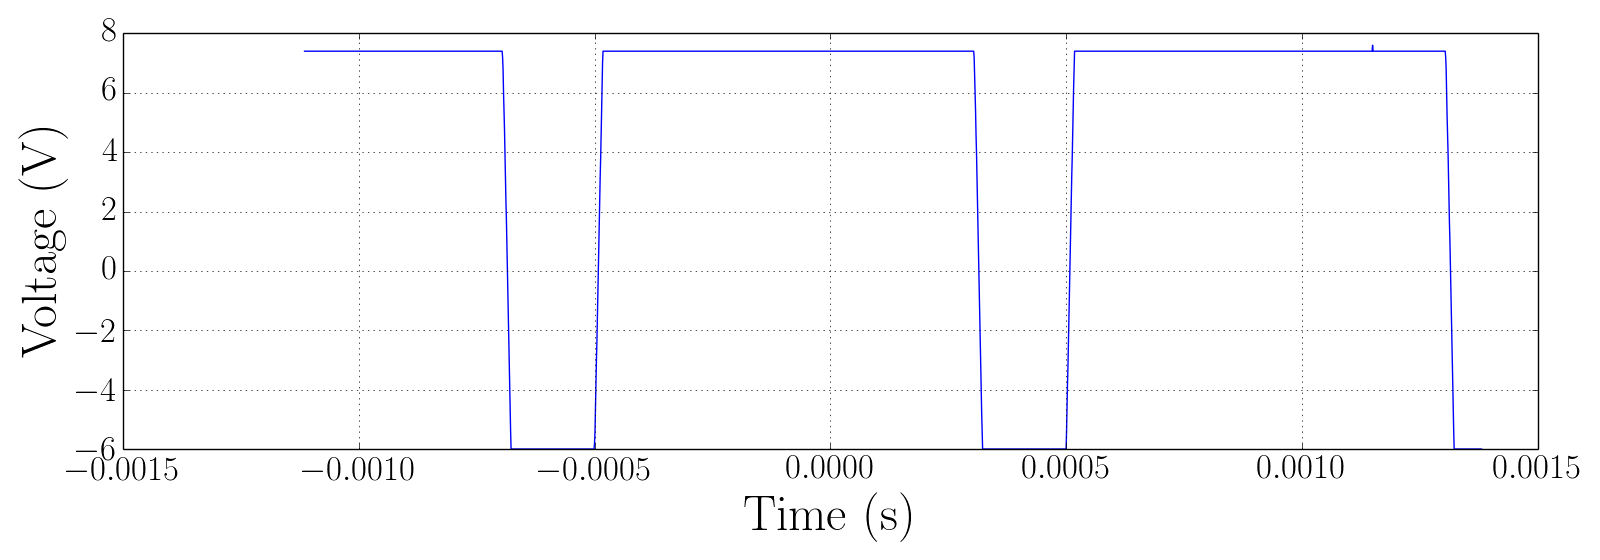
\includegraphics[scale=.22]{day1_lab8/ALL0002/F0002CH2}
  \captionof{figure}{a simple figure.}\label{fig:plot3}
\end{2colfig}

\labhead{7.2 Schmidt Trigger.}
{\bf a.} We used a potentiometer as $R_3 = \SI{25}{\kilo\ohm}$. $\pm V_{cc} = \pm \SI{8}{\volt}$.

\begin{2colfig}
  \center
  {\bf Comparator circuit.} \newline
  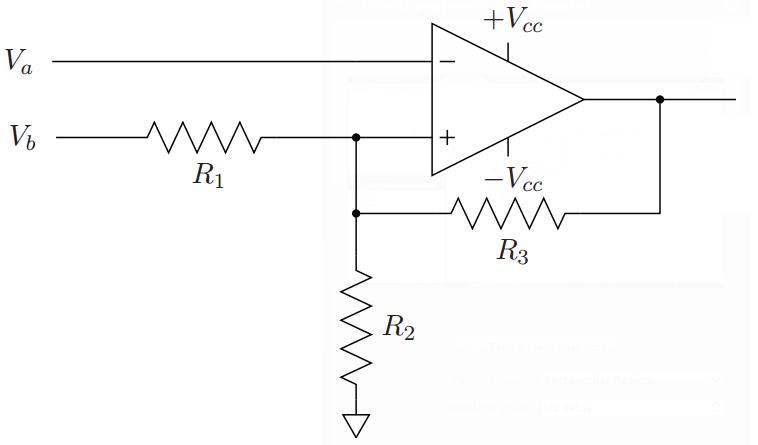
\includegraphics[scale=.4]{circuit2}
  \captionof{figure}{a simple figure. source: lab manual}\label{fig:circ2}
\end{2colfig}

{\bf b.} $V_a = \SI{10}{\volt}$ peak to peak ramp wave, at \SI{1}{\kilo\hertz}.
\newline

{\bf c.} Three screenshots, same as in part b, but we adjusted $R_3$ values to be: \SI{22.7}{\kilo\ohm}, \SI{1.7}{\kilo\ohm}, \SI{5.7}{\kilo\ohm} in that order. Symmetric sawtooth wave. Screenshots below.
\newline

\begin{2colfig}
  \center
  {\bf Input and output signals.} \newline
  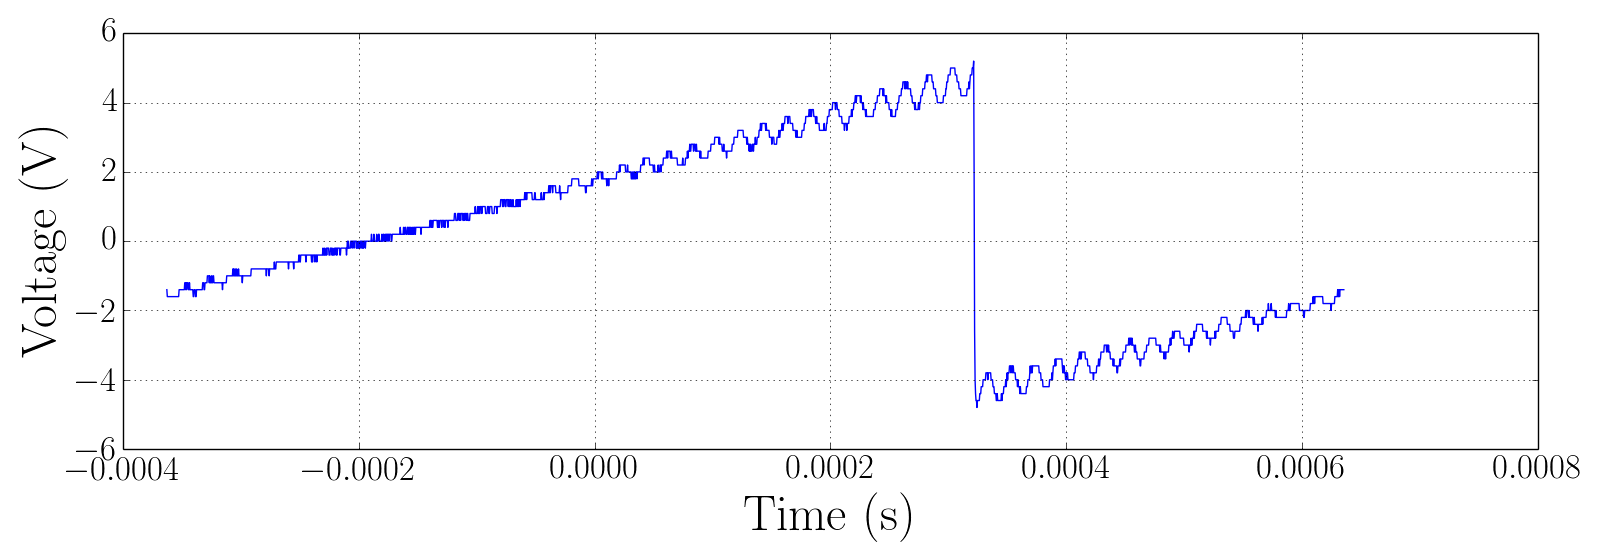
\includegraphics[scale=.22]{day1_lab8/ALL0003/F0003CH1}
  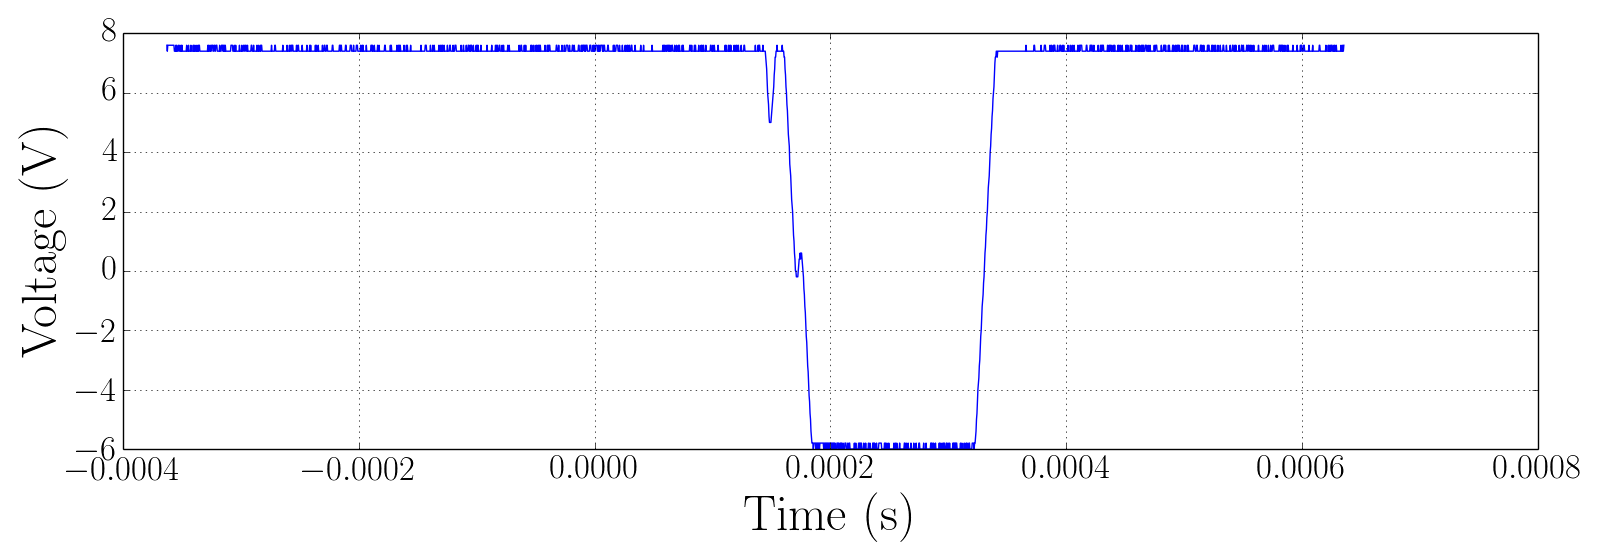
\includegraphics[scale=.22]{day1_lab8/ALL0003/F0003CH2}
  \captionof{figure}{a simple figure.}\label{fig:plot4}
\end{2colfig}

\begin{2colfig}
  \center
  {\bf Input and output signals.} \newline
  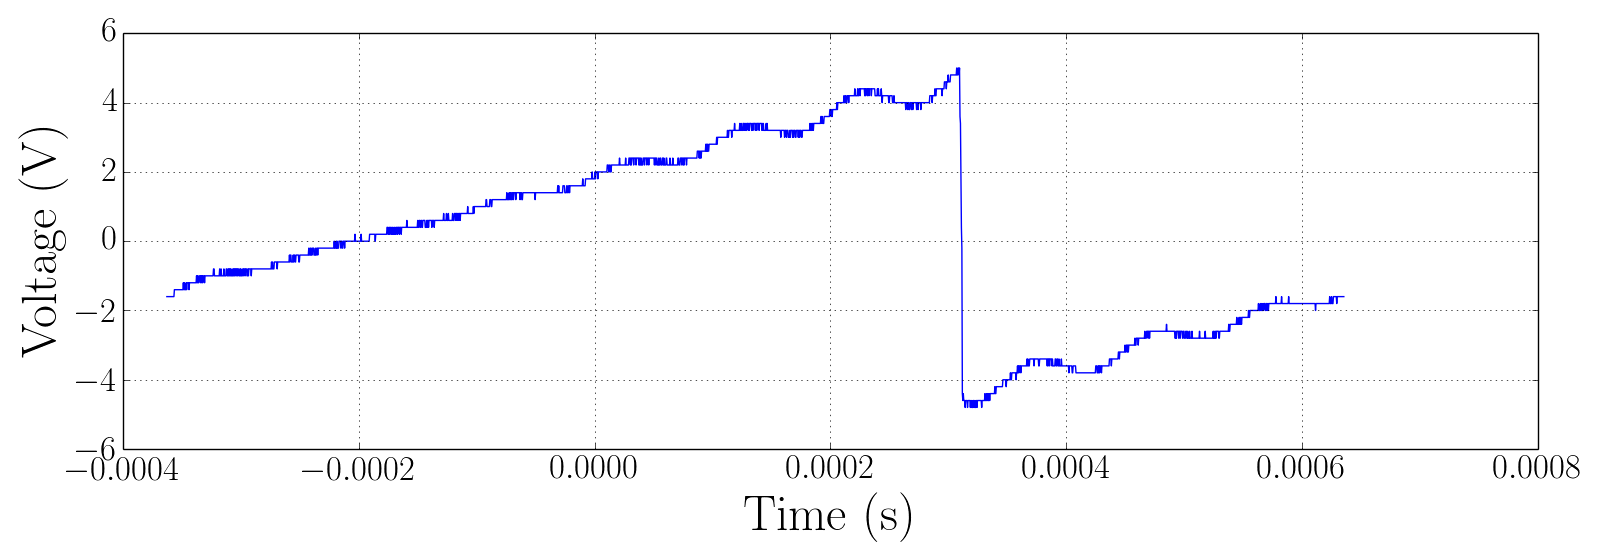
\includegraphics[scale=.22]{day1_lab8/ALL0004/F0004CH1}
  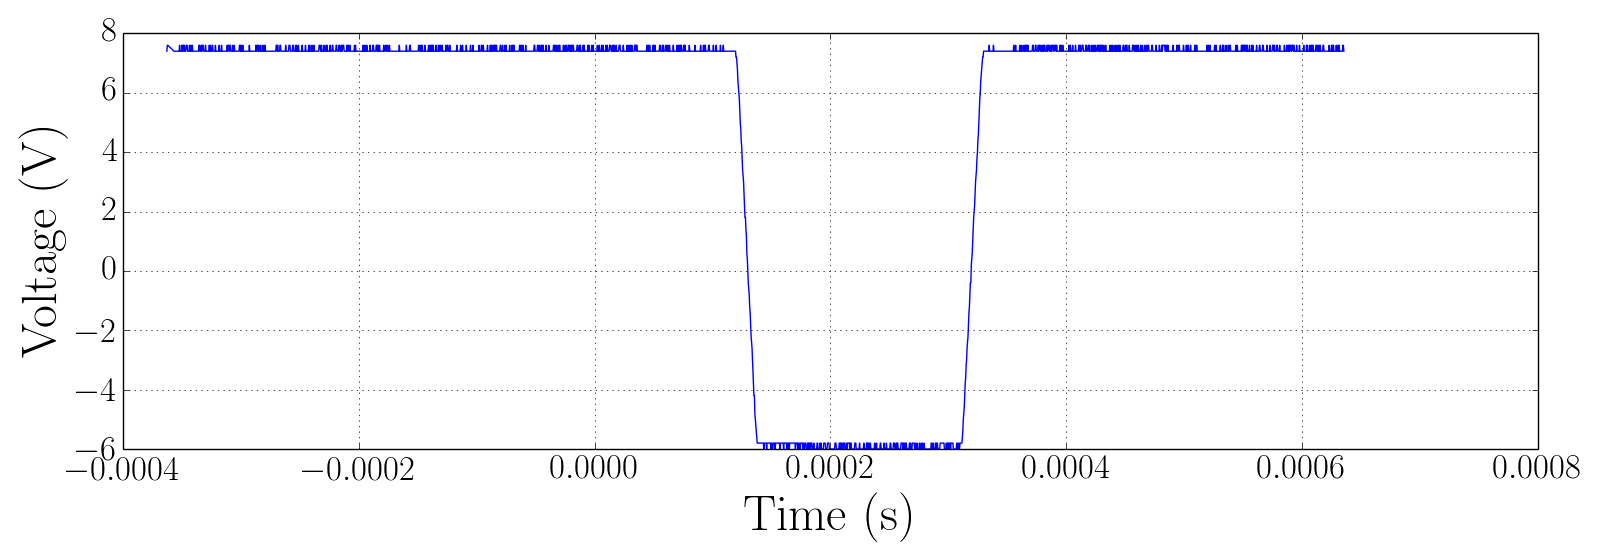
\includegraphics[scale=.22]{day1_lab8/ALL0004/F0004CH2}
  \captionof{figure}{a simple figure.}\label{fig:plot5}
\end{2colfig}

{\bf d.} Changed $R_2 = \SI{10}{\ohm}$. This lowered our reference voltage for the comparator. Screenshot below.
\newline

\labhead{7.3 Temperature Controller.} 
{\bf a.} We built the circuit. We wanted \SI{313}{\milli\volt} at
\SI{313}{\kelvin}, so $R_2 = \SI{30}{\ohm}, R_1 = \SI{928.4}{\ohm}$. Closest we could get was $R_2 = \SI{30}{\ohm}, R_3
= \SI{910}{\ohm}$. This gives us \SI{319}{\milli\volt} as our switch point (pre-schmidt trigger); good enough.
\newline

{\bf b.} For the schmidt trigger, we used $R_3 = \SI{130}{\kilo\ohm}$. From this, we obtain

\begin{gather}
  V_{high} = \SI{317}{\milli\volt}, \\
  V_{low} = \SI{320.55}{\milli\volt}.
\end{gather}

{\bf c.} Stuck a transistor in. Final circuit shown below.
\newline

\begin{2colfig}
  \center
  {\bf Comparator circuit.} \newline
  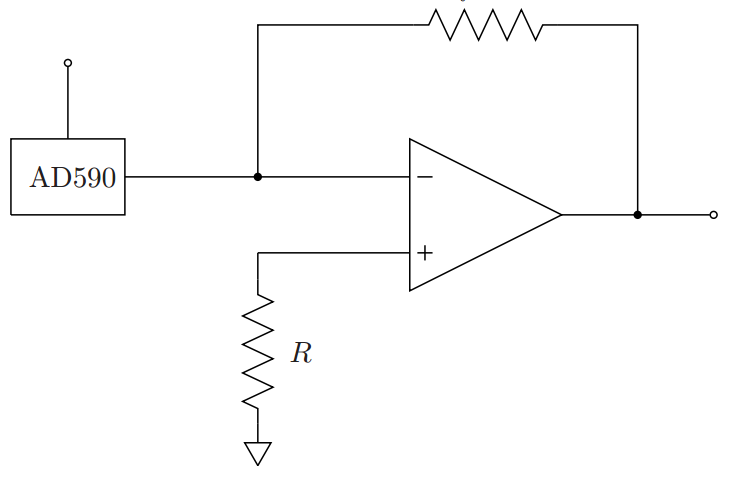
\includegraphics[scale=.4]{circuit3}
  \captionof{figure}{a work-in-progress figure. source: lab manual}\label{fig:circ3}
\end{2colfig}


And here's the scope trace.
\begin{2colfig}
  \center
  {\bf Input and output signals.}
  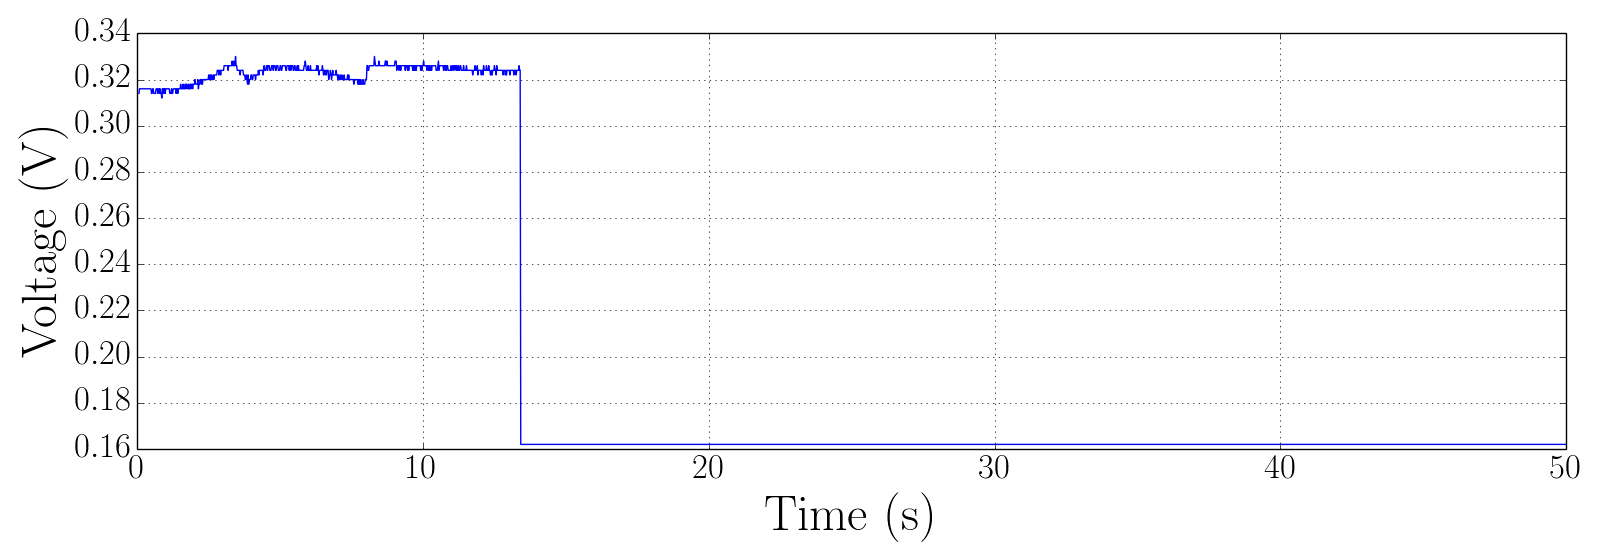
\includegraphics[scale=.22]{day3/ALL0006/F0006CH1}
  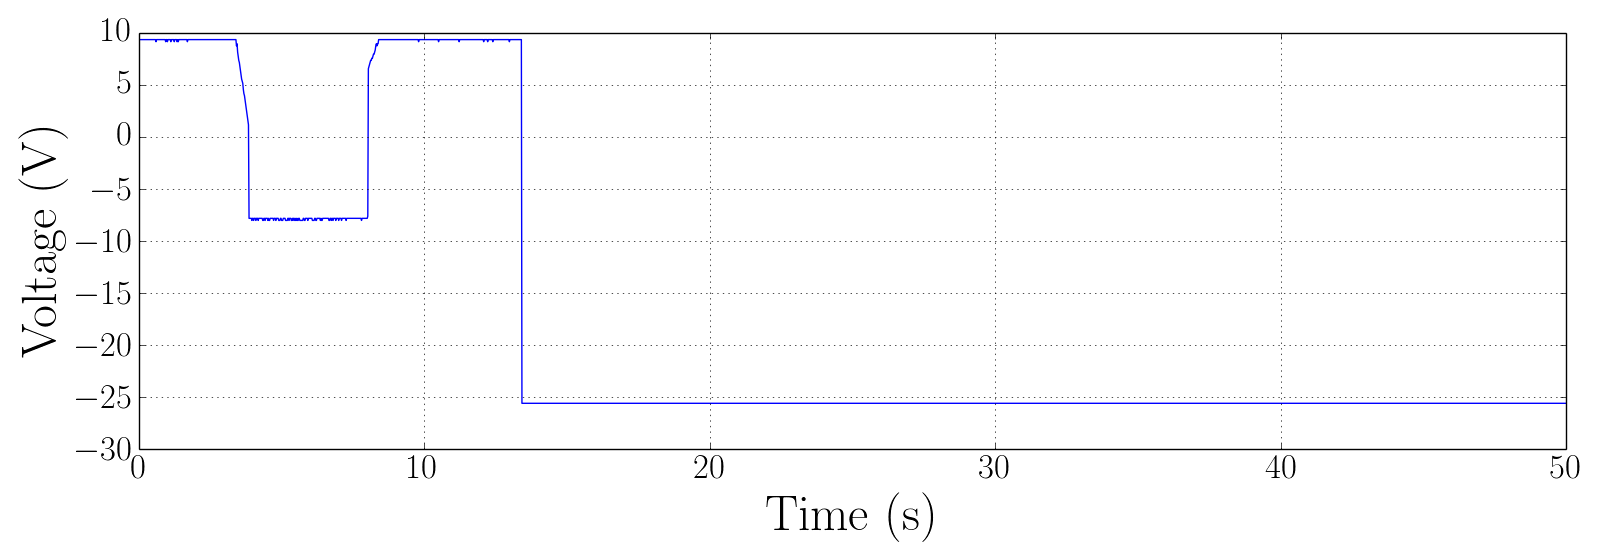
\includegraphics[scale=.22]{day3/ALL0006/F0006CH2}
  \captionof{figure}{a simple figure.}\label{fig:plot6}
\end{2colfig}
\end{multicols*}

\end{document}
